\documentclass[10pt, a4paper]{article}
\usepackage{lrec2006}
\usepackage{graphicx}
\usepackage{url}
\usepackage{ngerman}
\usepackage[utf8]{inputenc} \usepackage[pdftex]{hyperref}
\usepackage{fixltx2e}
\usepackage{tabularx}
\usepackage{natbib}
\usepackage{multibib}
\usepackage{pdfpages}

\newcites{net}{Internetquellen}

\newcommand{\myTitle}{Testgetriebene Entwicklung und kontinuierliche Integration
mit der SAP Mobile Platform\xspace} \newcommand{\myKeywords}{SAPUI5, OData,
Continuous Integration, Test-Driven-Development\xspace}
\newcommand{\mySubtitle}{\xspace}
\newcommand{\myDegree}{Bachelor of Science\xspace}
\newcommand{\myName}{Jan-Henrich Mattfeld, Maximilian Azimi\xspace}
\newcommand{\myMatrikel}{29866, 29287\xspace}
\newcommand{\myProf}{mgr\,inż. Alfred Schmidt\xspace}
\newcommand{\myCourse}{\xspace}
\newcommand{\myOtherProf}{\xspace}
\newcommand{\mySupervisor}{Dipl.-Wirt.-Inf.\,(FH)\,Christian Distelkamp\xspace}
\newcommand{\myFaculty}{\xspace}
\newcommand{\myDepartment}{Fachbereich\,2\xspace}
\newcommand{\myUni}{Hochschule Bremerhaven\xspace}
\newcommand{\myLocation}{Bremerhaven\xspace}
\newcommand{\myTime}{Oktober 2014\xspace}
\newcommand{\myVersion}{Version 1.0\xspace}

\title{Exposé\\--\\\myTitle}

\name{\myName}

\author{\myName\\
\myUni\\
\tt {jmattfeld,mazimi}@studenten.hs-bremerhaven.de}

\date{}

\address{\myUni\\
\{jmattfeld,mazimi\}@studenten.hs-bremerhaven.de\\}


\abstract{Mit aktuellen Tools und Frameworks wie SAPUI5, NW\,Gateway und SMP
bietet die SAP neue Möglichkeiten zur Entwicklung von geräteübergreifenden
mobilen Anwendungen. Diese wollen wir nutzen um Individualsoftware der abat\,AG
mobil nutzbar zu machen. Gleichzeitig sollen der Entwicklungs- und
Auslieferungsprozess automatisiert und entsprechende Tools erprobt werden.\\
\newline
\Keywords{\myKeywords}}

\hypersetup{ colorlinks=true, urlcolor=black, pdftitle={\myTitle},
pdfsubject={}, pdfauthor={\myName}, pdfproducer={}, pdfkeywords={\myKeywords},
pdfcreator={LaTeX},}

\begin{document}

\maketitleabstract

\section{Problemstellung}
Viele Projekte der abat\,AG arbeiten agil z.\,B. per Scrum.
Hierzu ist ein umfangreiches Projektmanagement-Tool als ABAP-Eigenentwicklung
vorhanden.

Dieses enthält allerdings weder ein Scrum-Board noch eine mobile Ansicht --
schneller Zugriff auf wichtige Funktionen ist unterwegs unmöglich. Die
Bearbeitung von Aufgaben ist nur am PC mit Intranet-Zugang möglich.

Aktueller Workflow: Ausdrucken der einzelnen Aufgaben, anpinnen, manuell
verschieben und parallel per Scrum-Transaktion in das SAP-System übertragen.

Dies gilt es mit aktuellen Technologien zu vereinfachen.

\section{Ziel}
Ziel ist eine geräteübergreifende App, die das Scrum-Board visualisiert und den
Zugriff auf Projektdaten schneller und einfacher gestaltet.
Während der Entwicklung sollen aktuelle Technologien und Tools zum Einsatz
kommen.
Kombiniert mit einem modernen Vorgehen, sollen Sicherheit und Zuverlässigkeit
besonders berücksichtigt werden.

In Zukunft sollen die Projektaufgaben mit Zusatzinfos auf einem Smartphone oder
Tablet angezeigt und bearbeitet werden können. Ein typischer Vorgang in dieser
App wäre die Statusänderung von Aufgaben -- Diese könnte dann per Drag and Drop
deutlich schneller erledigt werden.

Der bedeutendste Vorteil ergibt sich aus der ständigen Verfügbarkeit des
Projektstatus:
Das Scrum-Board muss nicht mehr physisch vorhanden sein, ein Blick in die App
genügt.
Der umständliche Zugriff über die alte, sehr umfangreiche SAP-Transaktion ist
dann nur noch selten nötig.

\section{Erkenntnisinteresse}
Besonders hervorzuheben ist die Kombination der verschiedenen Aspekte und
Vorgehen:

\begin{enumerate}
  \item Entwicklung einer aktuellen SAPUI5-App für ein bereits vorhandenes
  Altsystem auf ABAP-Basis.
  \item Die Integration des neuen NetWeaver Gateways und der entsprechenden
  OData-Services.
  \item Konsequente Nutzung des Frameworks (z.\,B. Logon- und
  Offline-Funktionen)
  \item Erstellung von Testfällen anhand der Spezifikation.
  \item Zuverlässigkeit vorhandener Features nach Updates durch automatische
  Regressionstests.
  \item Automatische Bereitstellung neuer App-Versionen für
  verschiedene Gerätetypen.
\end{enumerate}

Für alle folgenden Projekte werden diese Aspekte essentiell sein: Es gilt eine
entsprechende Toolchain zu erproben und zu etablieren, um
Softwarequalität und Erfüllung der Spezifikation nachhaltig zu gewährleisten.

\section{Gliederung (vorläufig)}
\begin{enumerate}
  \item Zusammenfassung
  \item Inhaltsverzeichnis
  \item Weitere Verzeichnisse
  \item Glossar
  \item Einführung
  \begin{enumerate}
    \item Motivation
    \item Aufgabenstellung
    \item Rahmenbedingungen
    \item Zielsetzung
  \end{enumerate}
  \item Grundlagen (aktueller Stand)
  \begin{enumerate}
    \item Test Driven Development
    \item Continuous Integration
    \item SAP \& Mobile
  \end{enumerate}
  \item Anforderungsanalyse
    \begin{enumerate}
    \item Spezifikation
    \item Testfälle
    \item Aufwandsschätzung
    \item Architektur
    \item Evaluierung JavaScript-Testframework
  \end{enumerate}
  \item Implementierung
  \begin{enumerate}
    \item CI-Toolchain
    \item SAPUI5-App
    \item Ergebnisse
  \end{enumerate}
  \item Schlussfolgerungen
  \begin{enumerate}
    \item Zusammenfassung
    \item Bewertung der Vorgehensweisen, Technologien und Tools
    \item Kritische Reflexion, Lessons Learned
    \item Fazit
    \item Ausblick
  \end{enumerate}
  \item Anhänge
  \begin{enumerate}
    \item Literaturverzeichnis
    \item Lasten-/Pflichtenheft
    \item Beispielcode und Konfiguration
    \item Diagramme, Pläne
  \end{enumerate}
  \item Eigenständigkeitserklärung
\end{enumerate}

\section{Toolauswahl (vorläufig)}
\begin{description}
\item[SAPUI5]
ist das SAP Mobile Framwork auf jQuery-Basis zur Entwicklung
der App
\item[NetWeaver Gateway]
stellt den OData-Service für die App bereit, um auf
die Daten des SAP-Systems zuzugreifen
\item[SAP Mobile Platform]
erweitert die OData-Services um Offline-Funktionen
\item[Git] als Versionsverwaltung für Dokumentation, Konfiguration und
Quellcode
\item[Jenkins]
als automatisierte Test- und Deploymentumgebung,
in Verbindung mit verschiedenen Plugins für die jeweiligen Testszenarien und
den PhoneGap-Build
\item[PhoneGap]
bietet über einen Hybrid-Container auf allen
aktuellen Mobilplattformen direkten Zugriff auf native Funktionen
\item[JSLint]
zur Qualitätssicherung des JavaScript-Codes
\item[JavaScript-Testframework]
wird während der Arbeit evaluiert
\item[Selenium]
für die Automatisierung der GUI-Tests
\end{description}

% Literaturverzeichnis
\renewcommand{\refname}{Literatur}
\bibliographystyle{natdin}
\bibliography{literatur}
\nocite{*} % Gibt alle Literaturangaben ohne Zitat aus.

% Verzeichnis der Internetquellen
\bibliographystylenet{natdin}
\bibliographynet{internet}
\nocitenet{*}

\clearpage
\section{Projektplan \& Aufgabenverteilung}
\begin{figure}[h]
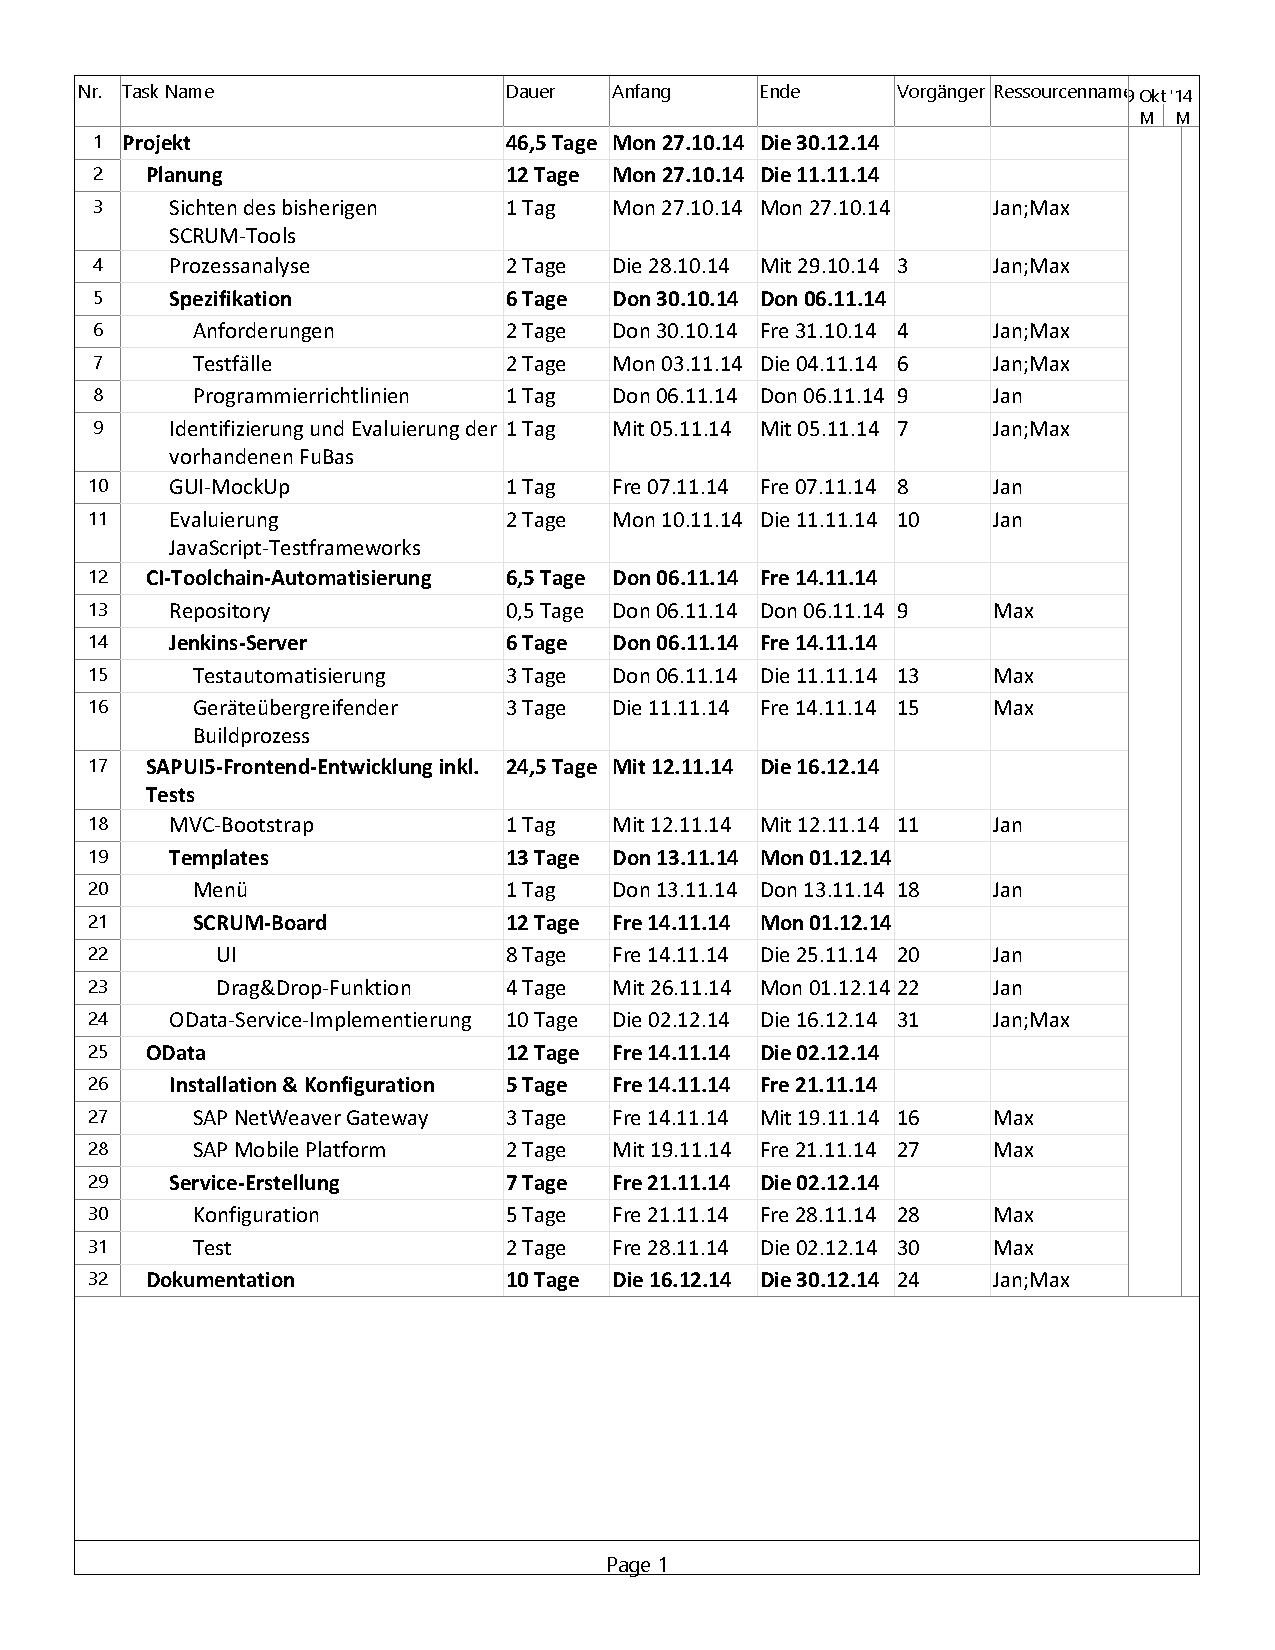
\includegraphics[trim = 13mm 60mm 31.7mm 13mm, clip, scale=0.9]{Zeitplan.pdf}
\caption{Gantt-Diagramm Projektablauf}
\label{fig:Projektablauf}
\end{figure}

\begin{tabular}{ll}
Jan & 46 Tage \\
Max & 46,5 Tage \\
\end{tabular}

\end{document}